\documentclass[12pt]{article}
\usepackage[utf8]{inputenc}
\usepackage{amsmath, amssymb}
\usepackage{hyperref}
\usepackage{tikz}
\usepackage[left=2.5cm,right=2.5cm,bottom=2.5cm]{geometry}
\usetikzlibrary{arrows.meta, positioning, bending}
\hypersetup{
    colorlinks=true}

\title{MATH 5707 (Spring 2026): Homework 4}
\date{}

\begin{document}
\vspace{-0.7in}

\maketitle
\vspace{-0.6in}


\section*{Directions and Introduction}
Submit a pdf of your solutions to the HW 4 assignment on Gradescope by 11:59 pm on February 27.

Problem 2 is marked as a peer review problem. \href{https://docs.google.com/document/d/1jSw9pmMJJFUx_6dTkcUi4k4HJNIrrIIgs9zdWhAycx0/edit?usp=sharing}{This document gives directions and deadlines for the peer review process.}

When working on this assignment, you should focus on showing fluency with the following skills:
\begin{itemize}
    \item Clearly communicate solutions using complete sentences and enough explanation that another 5707 student could follow your work.
   \item Write formal proofs about graph theoretic topics, including making sure your proofs meet the conventions of mathematical writing (see writing guidelines on Canvas).
    \item 
    Demonstrate fluency with the concept of spanning trees.
    \item Demonstrate fluency with the deletion/contraction algorithm.
   \item Write proofs involving trees. 
   \item Write a clear and correct proof of an if and only if statement. 
   \item Given two graphs, prove that they are isomorphic. 
   \item Given two graphs, prove that they are not isomorphic. 
\end{itemize}


\section*{Problems}

\begin{enumerate}
\item[0.] If you would like any of these problems to be graded for proficiency with the core skills, list the skill and the corresponding problem. 
  \item Consider the graph $G$ below.
  
  \begin{center}
    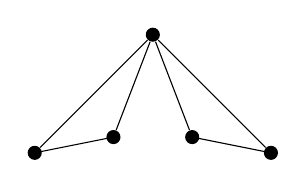
\begin{tikzpicture}
    \draw[every node/.style={inner sep=1.8pt,fill,circle}]
    (-1.5,-.2)node(x1){}--(-.5,0)node(x2){};
      \draw[every node/.style={inner sep=1.8pt,fill,circle}]
   (.5,0)node(x3){}--(1.5,-.2)node(x4){};
    \draw[every node/.style={inner sep=1.8pt,fill,circle}]
    (0,1.3)node(a){}
    \foreach \x in {1,2,3,4}{
    (a)--(x\x)};	
    \end{tikzpicture}
  \end{center}
  
  \begin{enumerate}
  \item Find all of the spanning trees of $G$.  Draw them all.
  \item Find two isomorphic trees from your set of spanning trees. Prove that they are, in fact, isomorphic. 
  \item Find two non-isomorphic trees from your set of spanning trees. Prove that they are not isomorphic. 
  \end{enumerate}
    \item  (2.2.2 from Bondy-Murty, peer review problem) (Each part will be worth 4 points and graded as a separate problem.) We define a \emph{cut edge} e in a graph $G$ to be an edge where $G-e$ has more connected components than $G$. \\Let $G=(V,E)$ be a connected graph and let $e\in E$.
    \begin{enumerate}
    \item Show that $e$ is in every spanning tree of $G$ if and only if $e$ is a cut edge of $G$.
    \item Show that $e$ is in no spanning tree of $G$ if and only if $e$ is a loop. 
    \end{enumerate}
    
     \item Consider the following weighted graph. 

\begin{center}
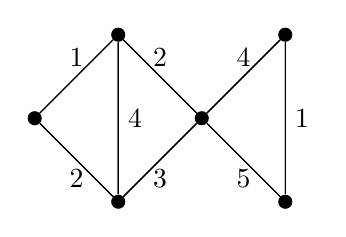
\begin{tikzpicture}[scale=1.5]
\draw[every node/.style={inner sep=1.8pt,fill,circle}]
(0,0) node(a){} -- ++(45:1) node(b){} -- ++(-45:1) node(c){} -- ++(45:1) node(x){}
(a) -- ++(-45:1) node(d){} -- (c) -- ++(-45:1) node(y){}  (b)--(d) 
(x)-- (y)
;
\draw
(x)-- node[right]{1} (y)
(a)-- node[above]{1} (b)
(b)-- node[above]{2} (c)
(c) -- node[below]{3} (d)
(d)-- node[below]{2}(a)
(d) -- node[right]{4}(b)
(c) --node[above]{4} (x)
(c) --node[below]{5} (y)
;
\end{tikzpicture}
\end{center}

\begin{enumerate}
\item Apply Kruskal's algorithm to find a minimum spanning tree in the graph. Show how the tree is created for each edge. In other words, include a series of pictures showing how the minimum spanning tree was created. 

\item Apply Prim's algorithm to find a minimum spanning tree in the graph. Show how the tree is created for each edge. In other words, include a series of pictures showing how the minimum spanning tree was created. 

\end{enumerate}

 \item  (2.4.1 from Bondy-Murty) Using deletion-contraction, evaluate $t(K_{3,3})$. 



\end{enumerate}

\end{document}